\documentclass{standalone}

\usepackage{tikz}
\usetikzlibrary{calc,decorations.markings}

\begin{document}

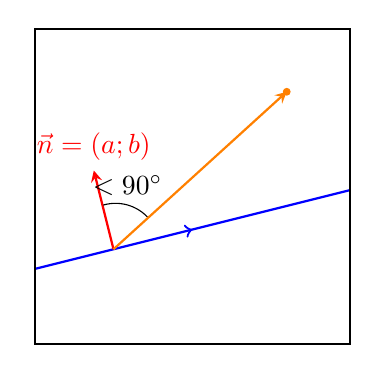
\begin{tikzpicture}[
  scale = 4,
  decoration={
      markings,
      mark=at position 0.5 with {\arrow{>}}}
  ]

\def\a{-0.25}
\def\b{1}
\def\xp{0.25}
\def\yp{0.3}
\def\c{\yp+(\a/\b)*\xp}
\coordinate (P) at (\xp,\yp);
\coordinate (Q1) at (0.8,0.8);
\coordinate (Q2) at (0.9,0.15);

\draw[blue, thick, postaction={decorate}] (0,{\c})--(1,{-(\a/\b)+\c});
\draw[red, thick, -stealth] (P)--++($0.25*(\a,\b)$) node[above] {$\vec n=(a;b)$};
\draw[fill=orange,orange] (Q1) circle (0.3pt);
\draw ($(P)+0.2*(Q1)-0.2*(P)$) arc(42.2737:106:0.14) node[midway, above] {$<90^{\circ}$};
\draw[orange,-stealth, thick] (P)--(Q1);
\draw[thick] (0,0) rectangle (1,1);

\end{tikzpicture}

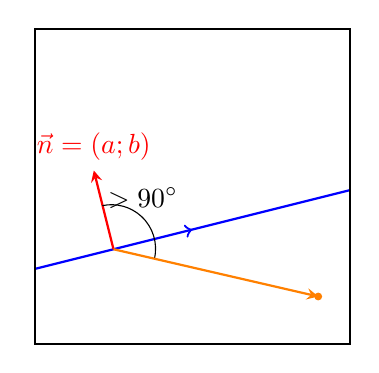
\begin{tikzpicture}[
  scale = 4,
  decoration={
      markings,
      mark=at position 0.5 with {\arrow{>}}}
  ]

\def\a{-0.25}
\def\b{1}
\def\xp{0.25}
\def\yp{0.3}
\def\c{\yp+(\a/\b)*\xp}
\coordinate (P) at (\xp,\yp);
\coordinate (Q1) at (0.8,0.8);
\coordinate (Q2) at (0.9,0.15);

\draw[blue, thick, postaction={decorate}] (0,{\c})--(1,{-(\a/\b)+\c});
\draw[red, thick, -stealth] (P)--++($0.25*(\a,\b)$) node[above] {$\vec n=(a;b)$};
\draw[fill=orange,orange] (Q2) circle (0.3pt);
\draw ($(P)+0.2*(Q2)-0.2*(P)$) arc(-12.9946:102:0.14) node[midway, above] {$>90^{\circ}$};
\draw[orange,-stealth, thick] (P)--(Q2);
\draw[thick] (0,0) rectangle (1,1);

\end{tikzpicture}

\end{document}